\documentclass{standalone}
\usepackage{tikz}
\usetikzlibrary{shapes.geometric, arrows.meta}

\tikzstyle{startstop} = [rectangle, rounded corners, minimum width=3cm, minimum height=1cm,text centered, draw=black, fill=red!30]
\tikzstyle{io} = [trapezium, trapezium left angle=70, trapezium right angle=110, minimum width=3cm, minimum height=1cm, text centered, draw=black, fill=blue!30]
\tikzstyle{process} = [rectangle, minimum width=3cm, minimum height=1cm, text centered, draw=black, fill=orange!30]
\tikzstyle{decision} = [diamond, minimum width=3cm, minimum height=1cm, text centered, draw=black, fill=green!30]
\tikzstyle{arrow} = [thick,->,>=stealth]

\begin{document}

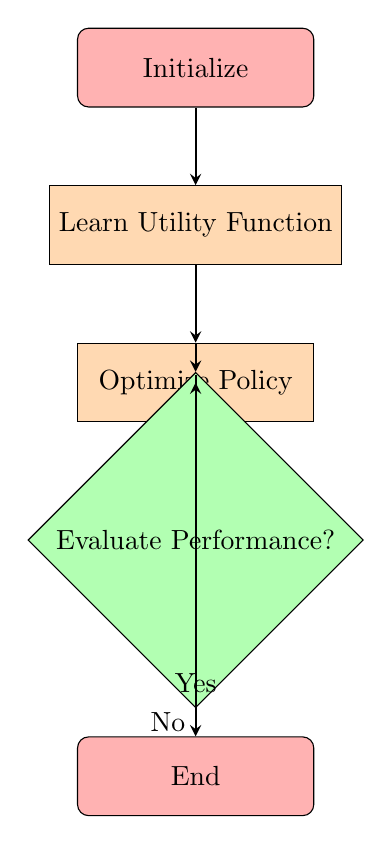
\begin{tikzpicture}[node distance=2cm]

\node (init) [startstop] {Initialize};
\node (learn) [process, below of=init] {Learn Utility Function};
\node (optimize) [process, below of=learn] {Optimize Policy};
\node (evaluate) [decision, below of=optimize] {Evaluate Performance?};
\node (end) [startstop, below of=evaluate, yshift=-1cm] {End};

% Drawing edges
\draw [arrow] (init) -- (learn);
\draw [arrow] (learn) -- (optimize);
\draw [arrow] (optimize) -- (evaluate);
\draw [arrow] (evaluate) -- node[anchor=east] {No} (end);
\draw [arrow] (evaluate) -- node[anchor=south] {Yes} ++(0,-2) |- (optimize);

\end{tikzpicture}

\end{document}